% -*- mode: fundamental -*-

% ****************************************************************

\chapter{Pending (to be written): Drum}

\markboth{Ch \arabic{chapter}: Pending (DRAFT)}{\copyrightnotice}

\setcounter{page}{1}
% \renewcommand{\thepage}{\arabic{page}}
\renewcommand{\thepage}{\arabic{chapter}-\arabic{page}}

\label{ch_Drum_Pending}

% ****************************************************************

This is a place-holder chapter with a TODO list of pending possible
topics to be written.

\begin{figure}[htbp]
  \centerline{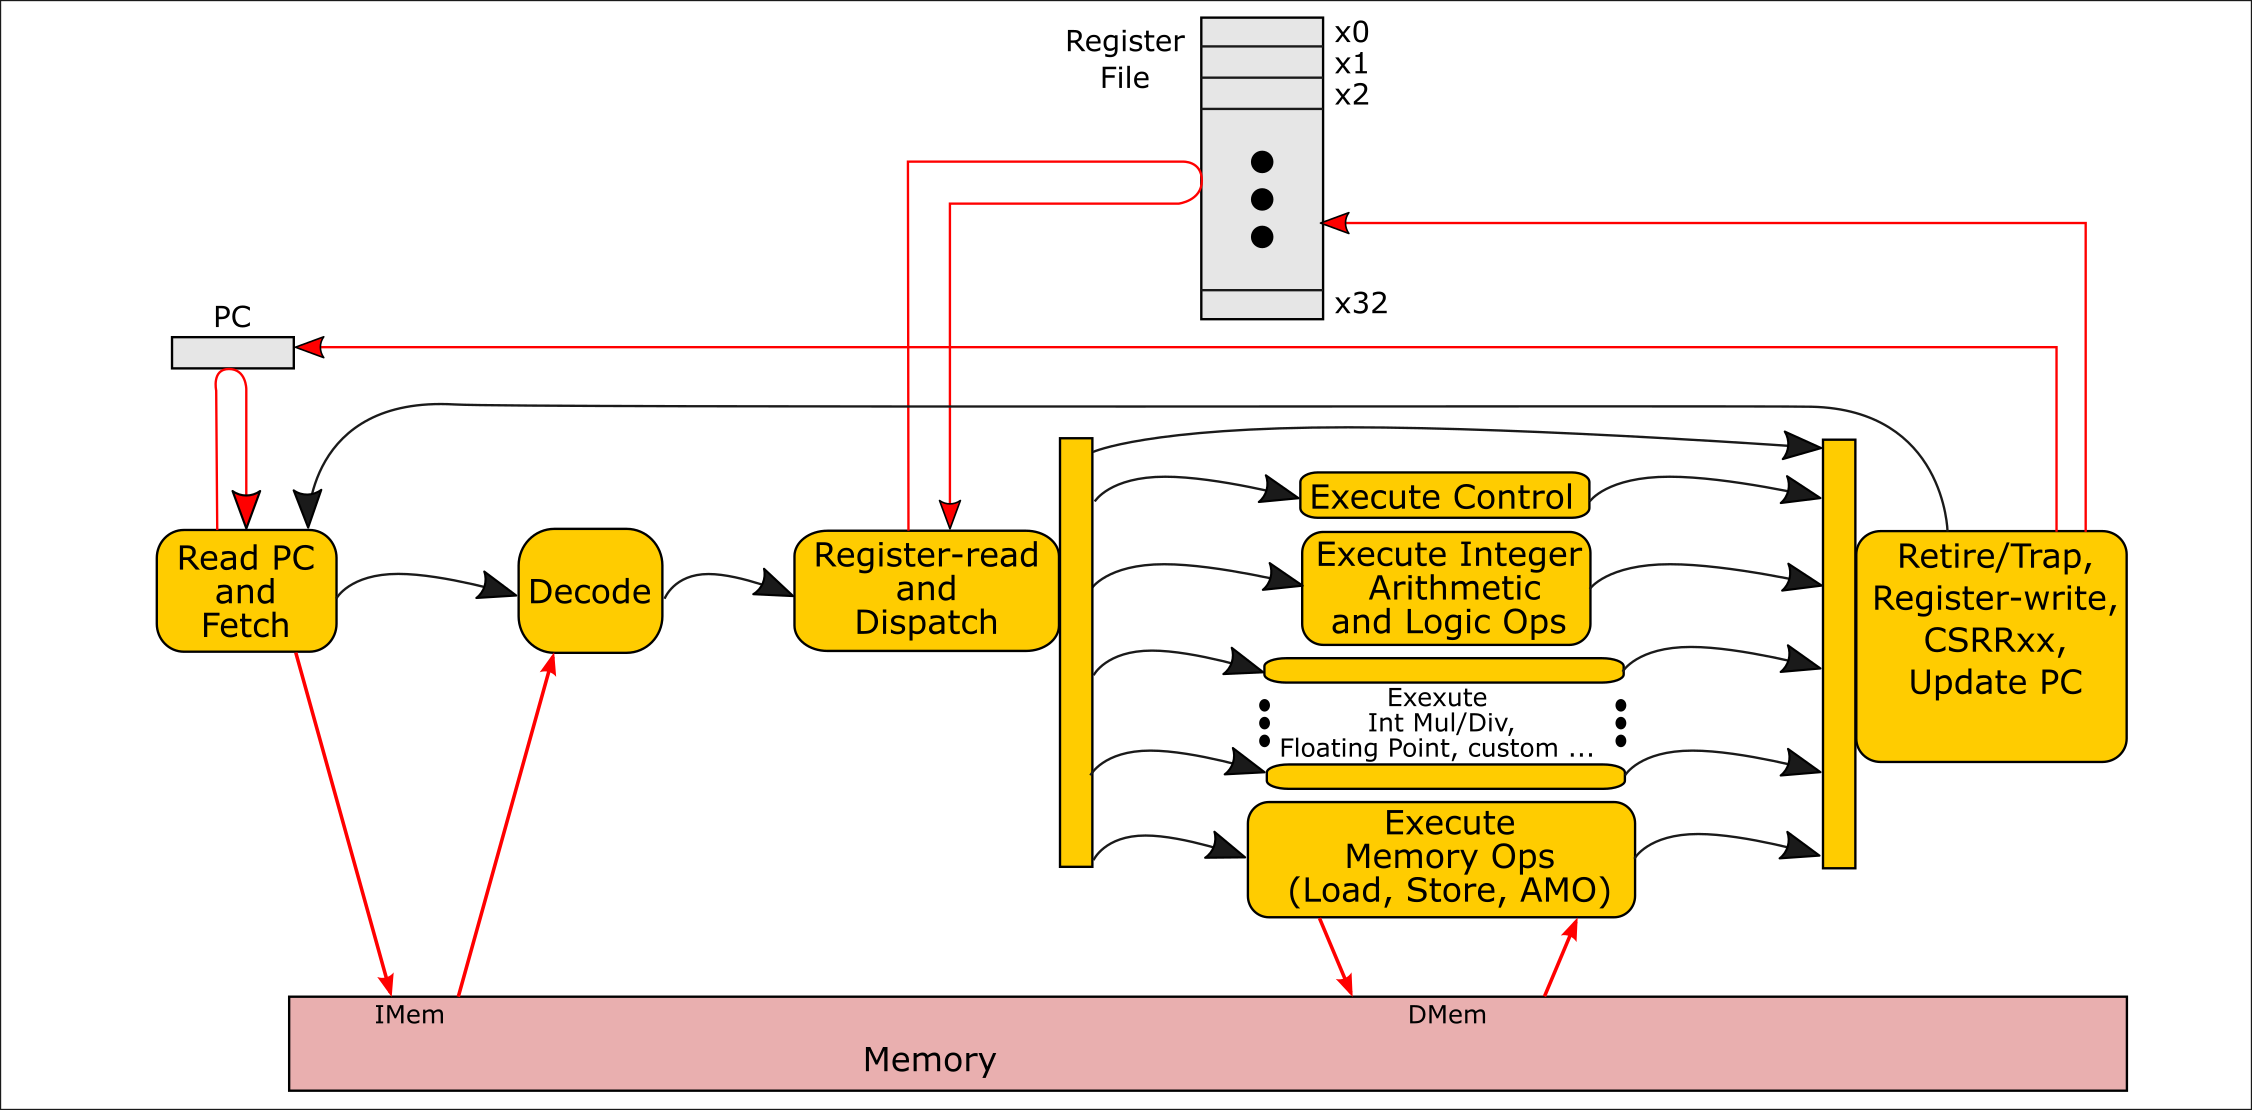
\includegraphics[width=6in,angle=0]{ch030_RISCV_Design_Space/Figures/Fig_Instr_Exec}}
  \caption{\label{Fig_Pending_Simple_Instr_Exec}Simple interpretation of RISC-V instructions (same as Fig.~\ref{Fig_Instr_Exec})}
\end{figure}

\hdivider

% ****************************************************************

\section{Drum: Remaining functions}

Register-read and write

EX IALU

DMem

Retire

% ****************************************************************

\section{Drum: Traps, and basic CSRs}

Note: These (implementation-independent) explanations may already be
done in Chapter~\ref{ch_ISA} on the RISC-V ISA:

\begin{tightlist}
  \item Explanation of illegal instruction traps
  \item Explanation of Fetch memory-access traps
  \item Explanation of LOAD/STORE/AMO memory-access traps
\end{tightlist}

Overview of how a trap is handled, using minimal set of CSRs (Control
and Status Registers): MCAUSE, MTVAL, MEPC, MTVEC, MCAUSE, MRET.

CSR register file and CSRRxx instructions to access them.

CSR (Control Status Registers)

% ****************************************************************

\section{Drum: Interrupts}

Interrupts in Drum:
\begin{tightlist}
  \item General concepts: MIP and MIE registers, MSTATUS.interrupt-enable-bit.

  \item Interrupts are initially disabled using the
        MSTATUS.interrupt-enable bit immediately; CSRxx can be used to
        re-enable.

  \item Interrupts are handled just like traps; the only question is:
        when to check for interrupts and respond.

  \item How does MIE bit return to 0?

\end{tightlist}

% ****************************************************************

\section{Measurements for Performance Analysis}

MTIME, MCYCLE, MINSTRET

``hpmcounter'' CSRs for other events.

% ****************************************************************
